\chapter{Esplorazione dei dati}
\label{exploration}

\section{Informazioni preliminari sul dominio}
Prima di addentrarci nell'analisi del nostro dataset, che si limita ad una categoria, abbiamo cercato delle visualizzazioni globali dell'intero marketplace Amazon. La Figura \ref{fig1} ci mostra una carattere fortemente stagionale: gli utenti sono molto più propensi a fornire recensioni nei periodi estivi, nonostante i picchi dei volumi di vendita si verifichino intorno al periodo natalizio \cite{trends}.
\par 

\begin{figure}[H]

  \centering
  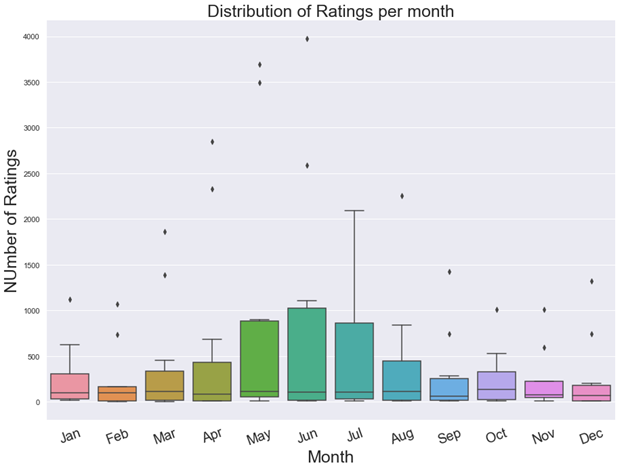
\includegraphics[width=0.95\linewidth]{figures/ext/1_monthly.png}
  \caption{General Amazon ratings per month \cite{plots1}}
    \label{fig1}
\end{figure}

La Figura \ref{fig2} visualizza invece il contributo di un utente, dandoci un'idea di quanto vocale sia la clientela Amazon, in media.

\begin{figure}[H]

  \centering
  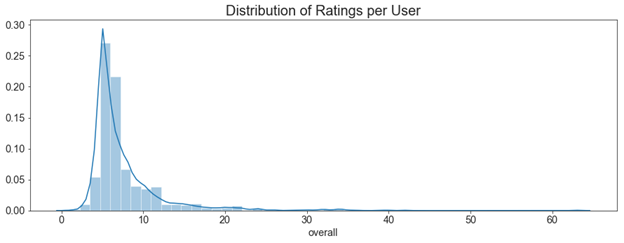
\includegraphics[width=1.1\linewidth]{figures/ext/1_peruser.png}
  \caption{General Amazon ratings per user \cite{plots1}}
  \label{fig2}
\end{figure}


\section{Descrizione dataset}
\label{descrizione_dataset}
Il dataset si presenta in formato JSON e viene caricato in memoria in un DataFrame con la libreria Pandas, molto efficiente per la gestione di dati voluminosi. 

La fase di caricamento e preprocessamento del dataset sono le più impegnative computazionalmente, impiegando gran parte del tempo totale.

Per ovviare a questo problema e muoverci più agevolmente durante lo sviluppo sfruttiamo la funzione \texttt{to\_pickle} di Pandas per salvare su disco una versione "cachata" del dataframe, abbreviando le successive esecuzioni della pipeline.

\par
Prima del salvataggio sono state effettuate alcune operazioni utili per rendere il dataset conforme agli obiettivi. In particolare:
\begin{itemize}
    \item Il campo \texttt{vote} è stato trasformato da tipo \texttt{object} a tipo \texttt{float}
    \item Il campo \texttt{reviewText} possedeva alcune recensioni vuote, inutili e perciò eliminate
\end{itemize}
Queste operazioni hanno ridotto il dataset portandolo da un totale di recensioni pari a 1128437 a un totale di 1127654, suddivise fra ben 157195 utenti e 48146 prodotti.
\begin{table}[H]
\small  
\centering
\begin{tabular}{|p{0.20\textwidth}||p{0.10\textwidth}||p{0.55\textwidth}|}
\hline
Campo & Tipo & Descrizione  \\
\hline
overall & int & Valutazione del prodotto (1-5)\\
verified & bool & Recensione proveniente da acquisto verificato\\
reviewTime & string & Data della recensione in formato string\\
reviewerID & string & Codice univoco del recensore\\
asin & string & Codice univoco del prodotto\\
style & string & Dizionario dei metadati del prodotto\\
reviewerName & string & Nome del recensore\\
reviewText & string & Testo della recensione\\
summary & string & Titolo della recensione\\
unixReviewTime & int & Data della recensione in formato unix\\
vote & float & Numero di voti della recensione \\
image & string & Immagine associata alla recensione\\
\hline
\end{tabular}
\caption{Campi del dataset con tipo e descrizione}
\label{table_dataset_description}
\end{table}

Il dataset possiede gli attributi mostrati in Tabella \ref{table_dataset_description}. Ogni record del dataset è la rappresentazione di una singola recensione svolta da parte di un utente per un certo prodotto nella data indicata. 
\par
Per l'identificazione dell'utente abbiamo a disposizione il campo \texttt{reviewerName} e il campo \texttt{reviewerID}: utilizzeremo solamente quest'ultimo per i nostri scopi.
Per quanto riguarda i campi relativi alla recensione, abbiamo a disposizione sia \texttt{summary} che \texttt{reviewText}.
\par
Per identificare il prodotto abbiamo a disposizione solamente il campo \texttt{asin}, che è un codice univoco da cui si può risalire a maggiori informazioni con l'utilizzo delle API Amazon o software di terze parti. 
\par
Le recensioni sono classificate come \textit{verificate} se provengono da un acquisto su Amazon per almeno l'80\% del valore originale dell'articolo. L'utente deve aver inoltre speso almeno 50\$ sul proprio account.

\section{Estensione del dataset}

A partire dal dataset originale abbiamo creato dei nuovi campi ritenuti di valore per effettuare una fase di esplorazione più approfondita. 

\subsection{Da \texttt{overall} a \texttt{opinion}}
\label{overall_opinion}
Osservando la distribuzione del campo \texttt{overall}, mostrata in Figura \ref{overall_distribution}, possiamo notare un forte sbilanciamento sul valore 5: questa tendenza è presente anche in dataset Amazon di categorie diverse dalla nostra.

\begin{figure}[H]
  \centering
  \includesvg[width=0.9\linewidth]{figures/1_overall_distribution}
  \caption{Overall distribution}
  \label{overall_distribution}
\end{figure}

In previsione della fase di sentiment analysis, il campo \texttt{overall} è stato utilizzato per la creazione del campo \texttt{opinion}, così composto:

\begin{itemize}
    \item I valori 1 e 2 vengono trasformati in \textit{negative}
    \item Il valore 3 viene trasformato in \textit{neutral}
    \item I valori 4 e 5 vengono trasformati in \textit{positive}
\end{itemize}

In Figura \ref{opinion_distribution} viene mostrata la distribuzione: essa è ovviamente simile a quella già osservata per il campo \texttt{overall} e sarà quindi necessario un bilanciamento del dataset per la fase di sentiment analysis.

\begin{figure}[H]
  \centering
  \includesvg[width=0.9\linewidth]{figures/1_opinion_distribution}
  \caption{Opinion distribution}
  \label{opinion_distribution}
\end{figure}

\subsection{Conteggio delle parole nelle recensioni}

Il campo \texttt{reviewText} è di fondamentale importanza per le fasi di sentiment e topic analysis. Ma per la fase di esplorazione, essendo il testo di una recensione un dato qualitativo, non è di alcun valore. Per questo motivo, abbiamo computato direttamente il numero di parole e creato il campo risultante \texttt{n\_words}. In Figura \ref{distribution_words_opinion} viene mostrata la distribuzione del campo \texttt{n\_words} rispetto al campo \texttt{opinion}, tenendo in considerazione solamente le recensioni con meno di 1000 parole per una questione di visibilità che sarebbe venuta meno considerando anche le (poche) recensioni composte da oltre 1000 parole.

\begin{figure}[H]
  \centering
  \includesvg[width=0.9\linewidth]{figures/1_correlation_words_opinion}
  \caption{Distribution of words in review for each opinion}
  \label{distribution_words_opinion}
\end{figure}

\subsection{Analisi temporale}
Il campo \texttt{unixReviewTime} fornisce la data della recensione in formato unix. Con alcune semplici manipolazioni del suddetto campo abbiamo creato i seguenti:

\begin{itemize}
    \item \texttt{month\_year} nel formato YYYY-MM
    \item \texttt{month} nel formato MM
    \item \texttt{year} nel formato YYYY
    \item \texttt{week\_day} in cui il giorno della settimana è rappresentato con un numero intero (0-6) 
\end{itemize}{}

Il dataset considera recensioni nell'arco di 16 anni circa: più precisamente la prima recensione risale al 23-10-2002, mentre l'ultima al 01-10-2018.
Considerato il dominio trattato, un'analisi di valore è quella di considerare la distribuzione delle recensioni tenendo in considerazione il giorno della settimana cosicché da mettere in risalto pattern di attività. \par 
Nel caso specifico, come è possibile osservare in Figura \ref{review_dist}, non vi è una dominanza degna di nota nonostante vi sia una tendenza a produrre meno recensioni nelle giornate di venerdì e sabato. 

\begin{figure}[H]
  \centering
  \includesvg[width=0.9\linewidth]{figures/1_review_distribution_per_day}
  \caption{Review distribution per day}
  \label{review_dist}
\end{figure}

\section{Prodotti più recensiti e recensori più popolari}
Il numero di utenti e di prodotti è nell'ordine delle migliaia (come anticipato nel Capitolo \ref{descrizione_dataset}) ed è impensabile anche solo immaginare di fare analisi esplorative approfondite su ogni singolo utente e su ogni singolo prodotto. Per questo motivo abbiamo deciso di focalizzare l'attenzione su un numero ristretto di utenti e di prodotti. 

\par

La Figura \ref{opinion_bestseller_products} mostra i 20 prodotti più popolari in termini di recensioni. Possiamo notare come, seppur ogni prodotto abbia perlopiù un maggior numero di recensioni \textit{positive}, per alcuni prodotti in particolare la percentuale di recensioni \textit{neutrali} e \textit{negative} è elevata rispetto alla distribuzione osservata nel Capitolo \ref{overall_opinion}. 

\begin{figure}[H]
  \centering
  \includesvg[width=0.9\linewidth]{figures/1_sentiment_reviews_bestseller_products}
  \caption{Opinion for bestseller products}
  \label{opinion_bestseller_products}
\end{figure}

\par
La Figura \ref{reviewers_most_reviews} mostra i 50 utenti con più recensioni prodotte, mentre la Figura \ref{opinion_top_reviewers} mostra la distribuzione delle valutazioni delle recensioni effettuate. Possiamo notare come la maggior parte degli utenti considerati dia in percentuale una valutazione in linea con la distribuzione osservata nel Capitolo \ref{overall_opinion}, fatta eccezione per casi estremi.

\begin{figure}[H]
  \centering
  \includesvg[width=1\linewidth]{figures/1_reviewers_most_reviews}
  \caption{Reviewers with most reviews}
  \label{reviewers_most_reviews}
\end{figure}

\begin{figure}[H]
  \centering
  \includesvg[width=1\linewidth]{figures/1_opinion_top_reviewers}
  \caption{Opinion of top reviewers}
  \label{opinion_top_reviewers}
\end{figure}

\section{Natura delle recensioni}
Il campo \texttt{verified} merita una trattazione dettagliata per capire se le recensioni \texttt{non verificate} sono di valore tanto quanto le recensioni \textit{verificate}. In Figura \ref{ver_unver_overall} si può notare che la distribuzione del campo \textit{overall} è praticamente identica.

\begin{figure}[H]
    \centering
    \subfigure[Unverified overall distribution]{\includesvg[width=0.4\linewidth]{figures/1_unverified_overall_distribution}} 
    \subfigure[Verified overall distribution]{\includesvg[width=0.4\linewidth]{figures/1_verified_overall_distribution}}
    \caption{Verified - Unverified overall distribution}
    \label{ver_unver_overall}
\end{figure}

In Figura \ref{ver_unver_toprev} è invece possibile notare una particolarità. Come in Figura \ref{opinion_top_reviewers} abbiamo preso i 50 utenti con più recensioni prodotte e la maggior parte delle loro recensioni risulta come \textit{non verificata}.
\par
Alcune riflessioni sono possibili soffermandoci su questa Figura. Come specificato nel Capitolo \ref{descrizione_dataset}, le recensioni sono classificate come \textit{verificate} se provengono da un acquisto su Amazon per almeno l'80\% del valore originale dell'articolo. Una suggestione potrebbe far propendere per l'idea che molti di questi utenti siano i cosiddetti \textit{top recensori} solitamente posizionati in cima alla lista dei commenti che (in teoria) non acquistano direttamente i prodotti recensiti che invece gli vengono prestati per provare il prodotto e scrivere una recensione imparziale.

\begin{figure}[H]
  \centering
  \includesvg[width=1\linewidth]{figures/1_verified_unverified}
  \caption{Verified - Unverified reviews of top reviewers}
  \label{ver_unver_toprev}
\end{figure}

\section{Correlazioni temporali e relative al traffico}

Aggregando temporalmente i dati abbiamo ottenuto alcuni grafici che suggeriscono correlazioni interessanti: la Figura \ref{figtime1} ci mostra come grande parte del traffico attivo sulle recensioni (ovvero gli utenti che votano e danno rilevanza alle recensioni esistenti) si distribuisce su quelle già più popolari, mentre la grande rimanenza rimane quasi intoccata da grossi picchi di attività di questo tipo.

\begin{figure}[H]

  \centering
  \includesvg[width=1.1\linewidth]{figures/1_avg_help_25_100_traffic}
  \caption{Average "helpfulness" of 25 and 200 most relevant reviews over time and traffic}
    \label{figtime1}
\end{figure}

\par

La Figura \ref{figtime2} mostra un fenomeno interessante: nonostante la quantità di recensioni cambi notevolmente nel tempo, la quantità di recensioni non verificate in rapporto al totale sembra rimanere (quasi) invariata, suggerendo un qualche tipo di moderazione.

\begin{figure}[H]

  \centering
  \includesvg[width=1.1\linewidth]{figures/1_ver_unver_time_traffic.svg}
  \caption{Verified - Unverified reviews over time and traffic}
  \label{figtime2}
\end{figure}


\par

Incrociando la lunghezza media delle recensioni con il loro voto, abbiamo ottenuto la Figura \ref{figtime3}. Con il passare del tempo (e l'aumentare vertiginoso del traffico) le recensioni sono generalmente più lunghe e meno generose con la valutazione che esprimono.

\par

Basandosi su alcuni di questi aspetti, Amazon ha sviluppato un modello di apprendimento automatico per assegnare un valore di rilevanza alle recensioni, in modo da poterle mettere in primo piano. In particolare, i fattori considerati sono: punteggio "utilità" della recensioni (voti), recensione verificata/non verificata, età della recensione.

\par 
Non è noto nel dettaglio come funzioni e in che modo questi fattori vengano pesati ma è certamente importante rilevare come un approccio di questo tipo permette ad Amazon di sfruttare i contributi degli utenti e capitalizzarci, promuovendo recensioni convincenti e prodotti che riescono a produrre (legittimamente o no, altro aspetto importante) feedback così positivi e virali.


\begin{figure}[H]

  \centering
  \includesvg[width=1.1\linewidth]{figures/1_rew_len_over_time.svg}
  \caption{Review length VS overall score over time}
  \label{figtime3}
\end{figure}

\newpage
\section{Polarizzazione delle valutazioni}

Uno degli aspetti fondamentali e poco chiaro delle recensioni è quanto esse siano polarizzate attorno un singolo voto numerico, in modo spesso estremo. È un fenomeno che si estende per ogni categoria di ogni marketplace in modo praticamente omogeneo.
Nel caso di Amazon, la gran parte delle recensioni riporta una valutazione numerica massima.
\par
In letteratura, abbiamo trovato un recente lavoro \cite{schoenmuller2018extreme} che investiga dettagliatamente la questione, descrivendo la \textit{polarity self-selection} come fattore trainante di questo fenomeno. È tendenza dei consumatori a recensire esperienze estreme. Si discute inoltre il fatto che le distribuzioni estreme di queste valutazioni ne riducono l'informatività, su larga scala.

\par
I seguenti grafici danno un'idea di questo comportamento: la figura \ref{disp1} confronta recensori abituali ed occasionali del sito Yelp, mostrando come utenti che producono più recensioni distribuiscono meglio le proprie valutazioni, senza esagerare con valutazioni massime nella maggior parte dei casi. \ref{disp2} affronta invece l'aspetto dell'incipit della recensione: quando siamo forzati a valutare un elemento, è più probabile che distribuiremo intro al 4 la nostra valutazione, mentre quando lasciamo una recensione di nostra spontanea volontà si tende a recensire ottime esperienze.

\begin{figure}[htbp]
  \centering
  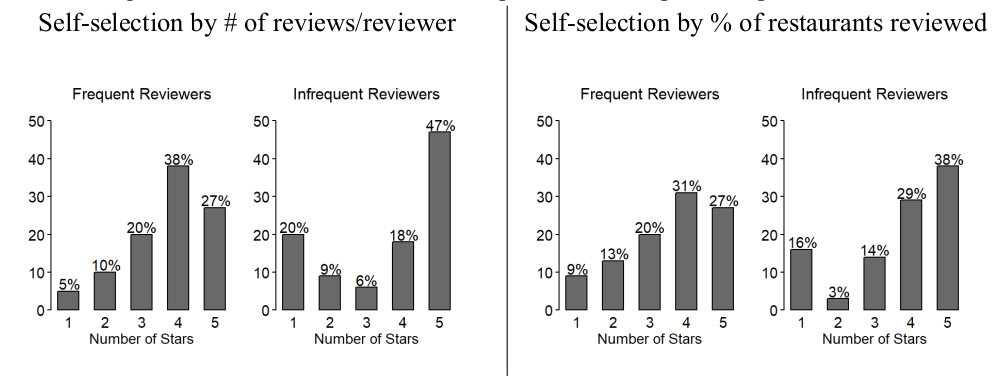
\includegraphics[width=1.1\linewidth]{figures/ext/1_frequentInfrequentYelp.png}
  \caption{Review Distribution of Frequent and Infrequent Yelp Reviewers \cite{schoenmuller2018extreme}}
  \label{disp1}
\end{figure}

\begin{figure}[htbp]
  \centering
  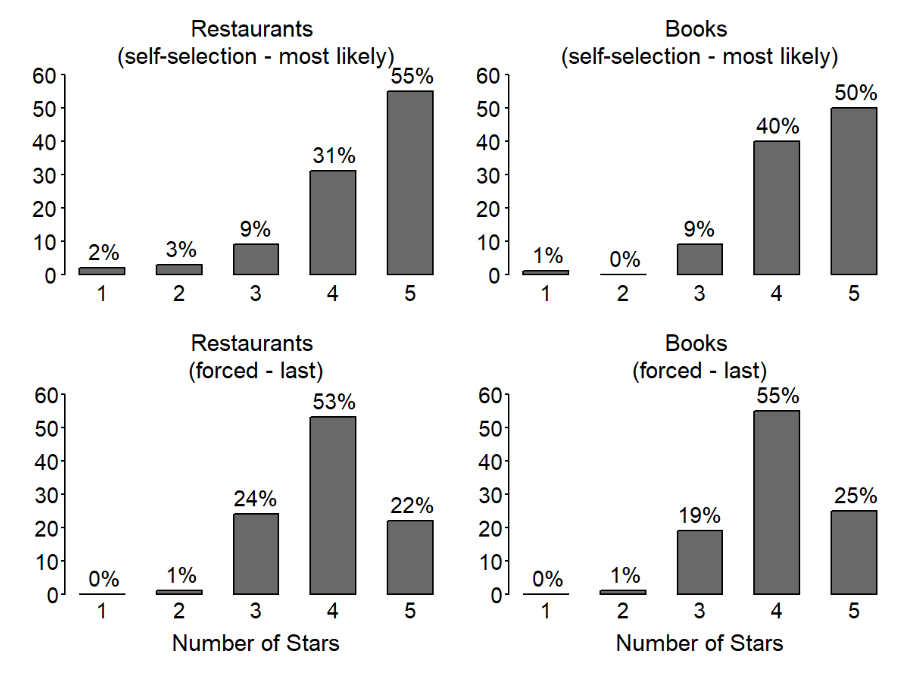
\includegraphics[width=1.1\linewidth]{figures/ext/1_selfVSforced.png}
  \caption{Empirical Distributions for Self-Selection versus Forced Reviews \cite{schoenmuller2018extreme}}
  \label{disp2}
\end{figure}